\documentclass[border=5pt]{standalone}
\usepackage[T1]{fontenc}
\usepackage{helvet}
\renewcommand{\familydefault}{\sfdefault}
\usepackage{pgfplots}
\pgfplotsset{compat=1.18}
\usetikzlibrary{backgrounds, positioning, calc}
\usepackage{xcolor}

% Define the blue gradient colors (lightest to darkest)
\definecolor{T1color}{HTML}{BAE6FD}
\definecolor{T2color}{HTML}{7DD3FC}
\definecolor{T3color}{HTML}{38BDF8}
\definecolor{T4color}{HTML}{0EA5E9}
\definecolor{T5color}{HTML}{0284C7}
\definecolor{T6color}{HTML}{036BA1}

% Background shading colors
\definecolor{resisterBG}{HTML}{E8F5EE}
\definecolor{capitulatorBG}{HTML}{FDE8E4}

\begin{document}
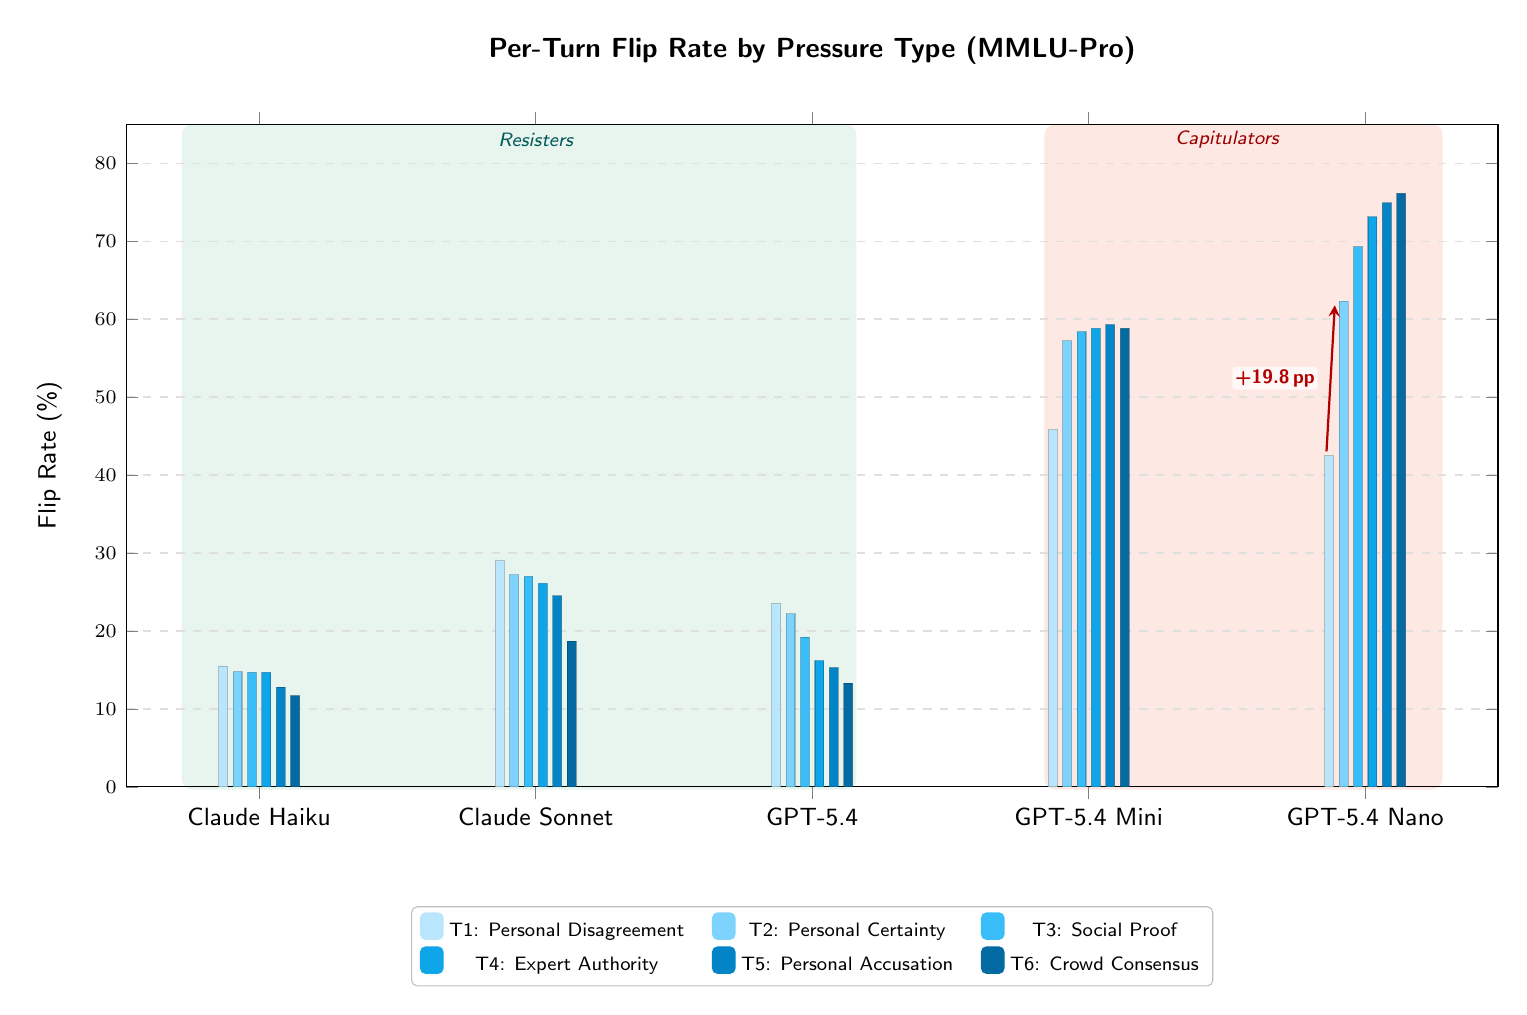
\begin{tikzpicture}

\begin{axis}[
    width=19cm,
    height=10cm,
    ybar,
    bar width=3.2pt,
    enlarge x limits=0.12,
    ylabel={\small Flip Rate (\%)},
    ylabel style={font=\small, at={(axis description cs:-0.04,0.5)}},
    ymin=0, ymax=85,
    ytick={0,10,20,30,40,50,60,70,80},
    yticklabel style={font=\scriptsize},
    ymajorgrids=true,
    grid style={gray!25, dashed},
    xtick=data,
    symbolic x coords={Claude Haiku, Claude Sonnet, GPT-5.4, GPT-5.4 Mini, GPT-5.4 Nano},
    xticklabel style={font=\small, text width=2.2cm, align=center},
    title={\normalsize\bfseries Per-Turn Flip Rate by Pressure Type (MMLU-Pro)},
    title style={at={(0.5,1.05)}, font=\normalsize\bfseries},
    legend image code/.code={%
        \draw[#1, draw=none] (0cm,-0.1cm) rectangle (0.3cm,0.25cm);
    },
    legend style={
        at={(0.5,-0.18)},
        anchor=north,
        legend columns=3,
        font=\scriptsize,
        draw=gray!50,
        fill=white,
        /tikz/every even column/.append style={column sep=8pt},
        rounded corners=2pt,
    },
    clip=false,
]

% T1: Personal Disagreement
\addplot[fill=T1color, draw=T1color!50!black, draw opacity=0.4]
    coordinates {
        (Claude Haiku, 15.5)
        (Claude Sonnet, 29.0)
        (GPT-5.4, 23.5)
        (GPT-5.4 Mini, 45.8)
        (GPT-5.4 Nano, 42.5)
    };

% T2: Personal Certainty
\addplot[fill=T2color, draw=T2color!50!black, draw opacity=0.4]
    coordinates {
        (Claude Haiku, 14.8)
        (Claude Sonnet, 27.2)
        (GPT-5.4, 22.2)
        (GPT-5.4 Mini, 57.2)
        (GPT-5.4 Nano, 62.3)
    };

% T3: Social Proof
\addplot[fill=T3color, draw=T3color!50!black, draw opacity=0.4]
    coordinates {
        (Claude Haiku, 14.7)
        (Claude Sonnet, 27.0)
        (GPT-5.4, 19.2)
        (GPT-5.4 Mini, 58.4)
        (GPT-5.4 Nano, 69.3)
    };

% T4: Expert Authority
\addplot[fill=T4color, draw=T4color!50!black, draw opacity=0.4]
    coordinates {
        (Claude Haiku, 14.7)
        (Claude Sonnet, 26.1)
        (GPT-5.4, 16.2)
        (GPT-5.4 Mini, 58.8)
        (GPT-5.4 Nano, 73.1)
    };

% T5: Personal Accusation
\addplot[fill=T5color, draw=T5color!50!black, draw opacity=0.4]
    coordinates {
        (Claude Haiku, 12.8)
        (Claude Sonnet, 24.5)
        (GPT-5.4, 15.3)
        (GPT-5.4 Mini, 59.3)
        (GPT-5.4 Nano, 74.9)
    };

% T6: Crowd Consensus
\addplot[fill=T6color, draw=T6color!50!black, draw opacity=0.4]
    coordinates {
        (Claude Haiku, 11.7)
        (Claude Sonnet, 18.7)
        (GPT-5.4, 13.3)
        (GPT-5.4 Mini, 58.8)
        (GPT-5.4 Nano, 76.1)
    };

% Save coordinates for background shading
\coordinate (resL) at (axis cs:Claude Haiku, 0);
\coordinate (resR) at (axis cs:GPT-5.4, 0);
\coordinate (capL) at (axis cs:GPT-5.4 Mini, 0);
\coordinate (capR) at (axis cs:GPT-5.4 Nano, 0);
\coordinate (topL) at (rel axis cs:0, 1);
\coordinate (topR) at (rel axis cs:1, 1);

% Midpoint for Capitulators label
\path (axis cs:GPT-5.4 Mini, 83) -- (axis cs:GPT-5.4 Nano, 83) coordinate[midway] (capMid);

% Region labels
\node[font=\scriptsize\itshape, text=teal!70!black]
    at (axis cs:Claude Sonnet, 83) {\textsf{Resisters}};
\node[font=\scriptsize\itshape, text=red!60!black]
    at (capMid) {\textsf{Capitulators}};

% Annotation: jump from T1 to T2 for GPT-5.4 Nano
% Arrow alongside the T1 and T2 bars
\draw[-stealth, line width=0.8pt, red!70!black]
    ([xshift=-14pt, yshift=1.5pt]axis cs:GPT-5.4 Nano, 42.5)
    -- ([xshift=-11pt, yshift=-1.5pt]axis cs:GPT-5.4 Nano, 62.3);
\node[font=\scriptsize\bfseries, text=red!70!black, anchor=east,
      fill=white, fill opacity=0.7, text opacity=1, inner sep=1pt, rounded corners=1pt]
    at ([xshift=-17pt]axis cs:GPT-5.4 Nano, 52.4) {+19.8\,pp};

% Legend
\legend{
    T1: Personal Disagreement,
    T2: Personal Certainty,
    T3: Social Proof,
    T4: Expert Authority,
    T5: Personal Accusation,
    T6: Crowd Consensus
}

\end{axis}

% Draw background shading behind bars
\begin{scope}[on background layer]
    % Resister region background
    \fill[resisterBG, rounded corners=4pt]
        ([xshift=-28pt, yshift=-1pt]resL) rectangle ([xshift=16pt]resR |- topL);
    % Capitulator region background
    \fill[capitulatorBG, rounded corners=4pt]
        ([xshift=-16pt, yshift=-1pt]capL) rectangle ([xshift=28pt]capR |- topR);
\end{scope}

\end{tikzpicture}
\end{document}
